\chapter{Vertical extent of the layers: partially filled containers}
\label{ch:partial}

\section{The idea}

A layer does not always fill the whole height of the sample. A powder or a liquid poured into a can leaves an
empty space above it; a powder can rest on a support inside the can; a can or a cell can start inside the beam,
so that part of the beam passes below it. \mcams\ describes all these cases with one property of every layer:
the \textbf{band of heights} that contains its material.

\begin{itemize}
  \item Layer $i$ contains material between its \textbf{bottom} $b_i$ and its \textbf{top} $t_i = b_i + h_i$,
        where $h_i$ is its \textbf{height}. Heights are lab coordinates $y$ in mm, measured from the
        \textbf{centre of the beam} ($y=0$; negative values are below it).
  \item Below $b_i$ and above $t_i$ the layer is \textbf{empty}: no attenuation and no interaction. Particles fly
        through the empty parts, so the beam can pass over or under the material, and scattered particles can
        cross the empty space before they enter another layer or leave the sample.
  \item A layer for which nothing is said fills the whole height of the sample, so every sample of the previous
        versions behaves exactly as before.
\end{itemize}
Each layer has its own band, so a can whose wall is full and whose powder rests on a support is just two layers
(Figure~\ref{fig:bandgeom}a). The same works for a flat cell (Figure~\ref{fig:bandgeom}b), for a round cell (disc, Chapter~\ref{ch:disc}),
for a spherical flask (Chapter~\ref{ch:sphere}) and for any number of layers.

\begin{note}[New in version 2.2]
In version 2.0 and 2.1 all the layers started at the bottom of the sample and only their level could change
(Figure~\ref{fig:partialgeom}). From version 2.2 the bottom of each layer is free. The older ways of describing
the filling (\code{fill_height} and \code{fullness}) are still accepted, with the same meaning
(Section~\ref{sec:legacy}).
\end{note}

\begin{figure}[H]
  \centering
  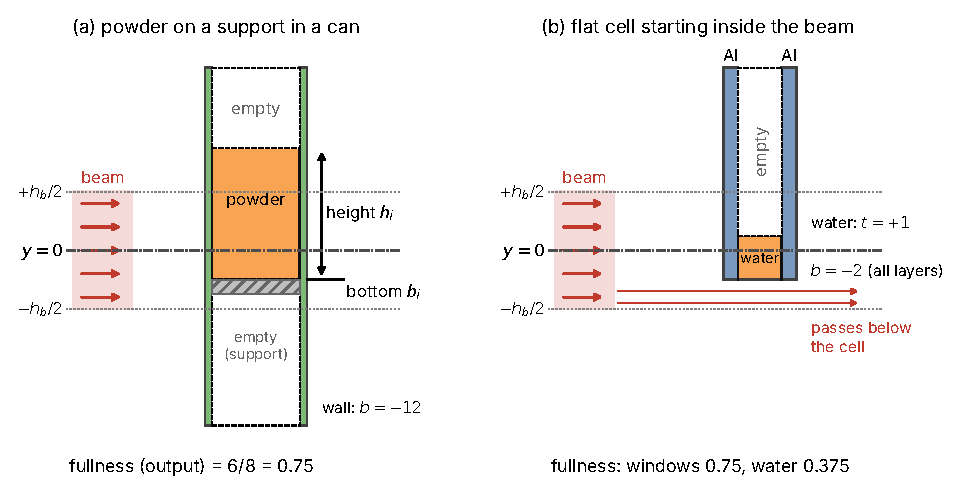
\includegraphics[width=\textwidth]{fig_band_geometry}
  \caption{Layers with their own band (version 2.2), side view. (a)~A powder resting on a support inside a can whose
  bottom is below the beam: the powder goes from $b=-2$ to $t=7$~mm, the wall from $-12$~mm upwards. (b)~A flat cell
  whose windows start inside the beam, at $y=-2$~mm: the lowest 2~mm of the beam pass below the cell. Above the material
  the layers are empty.}
  \label{fig:bandgeom}
\end{figure}

\section{Describing a layer: bottom and height}

The recommended description has two optional fields of \code{Layer}:
\begin{center}\small
\begin{tabular}{@{}lp{11.2cm}@{}}
  \toprule \textbf{Field} & \textbf{Meaning} \\ \midrule
  \code{bottom} & $b_i$: height $y$ of the bottom of the material, in mm from the centre of the beam. \code{None}: the bottom of the sample. \\
  \code{height} & $h_i\geq0$: height of the material in mm; the top is $t_i = b_i + h_i$. \code{None}: up to the top of the sample. \\ \bottomrule
\end{tabular}
\end{center}
\begin{lstlisting}
from toscana.corrections.mcams.sample_base import Layer
Layer("powder", 6.0, 0.25, 0.8, bottom=-2.0, height=9.0)   # from y = -2 to y = +7
Layer("V",      0.2, 0.073, 0.5, bottom=-12.0, height=30.0) # the can
{"name": "powder", "thickness": 6.0, "mu": 0.25, "bottom": -2.0, "height": 9.0}  # as a dict
\end{lstlisting}
The material is always limited to the sample: a band that goes beyond the bottom or the top of the sample is cut there.

\paragraph{Why bottom and height?} They are the two numbers that one measures on a real sample (where the powder
starts, and how high it is), they fix the geometry completely, and they describe the material \emph{outside} the
beam too. That material is not illuminated, but it scatters again the particles that leave the beam region, and it
changes the multiple scattering (Section~\ref{sec:partial-results}). Two other descriptions were possible and were
not chosen as the primary one:
\begin{itemize}
  \item \emph{bottom and top}: equivalent to bottom and height; the height is usually the number one knows (the
        amount of powder), and it cannot be negative by mistake.
  \item \emph{fullness}: one number cannot fix the band once the bottom is free ($f = 0.5$ may be the lower half of
        the beam, the upper half or a band in the middle), and it says nothing about the material outside the beam.
        The fullness is therefore an \textbf{output} of the sample: \code{sample.beam_fullness()}.
\end{itemize}

\section{The height of the sample}

The sample occupies $y_\mathrm{bottom}\leq y\leq y_\mathrm{top}$: the box of a slab, or the length of the cylinders.
It is given as before by \code{height} and \code{y_bottom}. With the layers described by their bands, it can also be
left out: with \code{height=None} the sample is the smallest range that contains the bands of all the layers given
with \code{bottom} and \code{height} (the \emph{envelope}), and \code{y_bottom} defaults to the lowest bottom.
\begin{lstlisting}
can = create_cylindrical_sample(None, [
    Layer("powder", 6.0, 0.25, 0.8,  bottom=-2.0,  height=9.0),
    Layer("V",      0.2, 0.073, 0.5, bottom=-12.0, height=30.0)],
    beam_height=8.0)             # sample from y = -12 to +18
\end{lstlisting}
A layer given without a band fills this envelope.

\section{Fullness: the fraction of the beam covered}

For a beam of height $h_b$ centred on $y=0$, the fullness of layer $i$ is the part of the beam height that its
material covers:
\begin{equation}
  f_i = \frac{\max\bigl(0,\ \min(t_i, h_b/2) - \max(b_i, -h_b/2)\bigr)}{h_b}.
  \label{eq:fullness-general}
\end{equation}
It is 1 if the material covers the whole beam, and 0 if the beam passes completely above or below it.
\code{sample.beam_fullness()} returns it for every layer (it needs the beam height, given when the sample is created
or as an argument), and \code{summary()} shows it in parentheses. With a uniform beam, the number of particles that
interact in a layer is proportional to $f_i$, wherever the band is (Example~10 and Figure~\ref{fig:bandpos}). This is
the value of \code{/fullness} in \textsc{correct}; the comparison with \textsc{pycorrect} shows when the correction of
\textsc{correct} based on it is exact.

\section{The forms of version 2.0}
\label{sec:legacy}

The level of the material can still be given relative to the bottom of the sample:
\begin{description}
  \item[Fill height $h$] (\code{fill_height}, or the 5th element of a tuple): material from the bottom of the sample up
        to $y_\mathrm{bottom}+h$. It is the same as \code{bottom=y_bottom, height=h}.
  \item[Fullness $f$] (\code{fullness}): material from the bottom of the sample up to the level $-h_b/2 + f\,h_b$, i.e.\
        covering the lower fraction $f$ of the beam. To turn it into a level the sample needs the beam height:
        create it with \code{beam_height=...}.
\end{description}
\code{bottom}/\code{height} cannot be combined with \code{fill_height}/\code{fullness} in the same layer; the layers of
one sample can use different forms.

\begin{figure}[H]
  \centering
  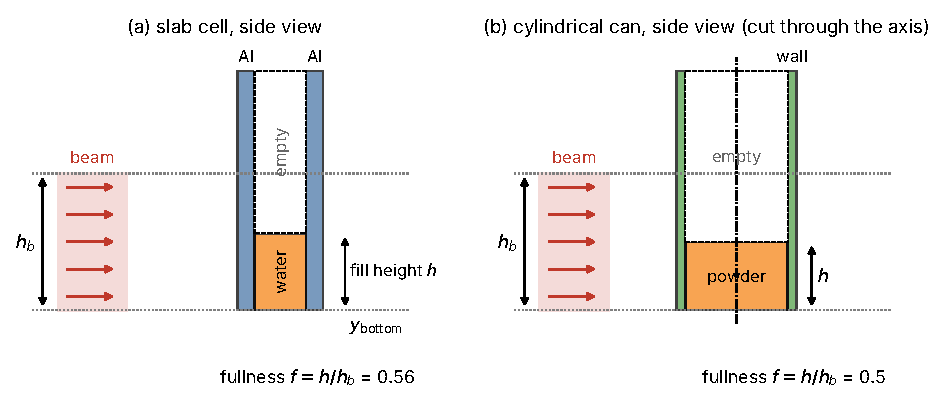
\includegraphics[width=\textwidth]{fig_partial_geometry}
  \caption{The description of version 2.0, side view. (a)~Flat cell: two aluminium windows (full) and water up to a
  fill height $h$. (b)~Cylindrical can: the wall is full and the powder reaches the height $h$. Here the bottom of the
  sample is at the bottom of the beam, so the fullness is simply $f=h/h_b$.}
  \label{fig:partialgeom}
\end{figure}

\begin{warn}[Fullness 1 means completely full]
A layer with \code{fullness=1} is taken as \emph{completely} full, up to the top of the sample, because the fullness
cannot tell how much material lies above the beam. Material above the beam is not illuminated, but it does scatter the
particles that leave the beam region upwards, and this increases the multiple scattering (Section~\ref{sec:partial-results}).
To fill a layer exactly up to the top of the beam, give \code{height} (or \code{fill_height}) instead.
\end{warn}

\section{Creating a sample}

The functions that build the samples accept \code{height=None} and two optional arguments:

\begin{fnbox}{create\_slab\_sample(width, height, layers, z\_front=0, plane\_angle\_deg=90, y\_bottom=None, beam\_height=None)}
\code{height}: height of the slab (mm), or \code{None} for the envelope of the layers.
\code{y_bottom}: height of the bottom of the sample (mm); default centred, or the lowest bottom of the layers.
\code{beam_height}: beam height (mm), needed for \code{fullness} and \code{beam_fullness()}.
\end{fnbox}
\begin{fnbox}{create\_cylindrical\_sample(height, layers, y\_bottom=None, beam\_height=None)}
The same arguments for concentric cylinders.
\end{fnbox}
\begin{fnbox}{make\_sample(geometry, layers, height=None, width=None, plane\_angle\_deg=90, y\_bottom=None, beam\_height=None)}
The factory passes them on to the geometry chosen.
\end{fnbox}

All the ways of writing a layer:
\begin{lstlisting}
from toscana.corrections.mcams.sample_base import Layer

Layer("water", 3.0, 0.56, 1.0, bottom=-2.0, height=3.0)    # 2.2: band from -2 to +1
{"name": "water", "thickness": 3.0, "mu": 0.56, "bottom": -2.0, "height": 3.0}
("water", 3.0, 0.56, 1.0, 4.0)                             # 2.0: fill height (5th element)
Layer("water", 3.0, 0.56, 1.0, fill_height=4.0)            # 2.0
Layer("water", 3.0, 0.56, fullness=0.5)                    # 2.0: lower half of the beam
\end{lstlisting}
Layers computed from their chemical formula (Chapter~\ref{ch:builder}) accept the same arguments:
\begin{lstlisting}
props = compute_layer_properties("D2O", 6.0, "D2O", 1.107, cross_sections={...})
props.as_layer(bottom=-2.0, height=9.0)  # Layer object
props.as_tuple(fill_height=4.0)          # 5-element tuple (version 2.0 form)
build_layer("D2O", 6.0, "D2O", 1.107, cross_sections={...}, bottom=-2.0, height=9.0)
\end{lstlisting}

\section{What the sample tells you}

\begin{center}\small
\begin{tabular}{@{}>{\raggedright\arraybackslash}p{5.2cm}p{9.6cm}@{}}
  \toprule \textbf{Attribute or method} & \textbf{Content} \\ \midrule
  \code{sample.summary()} & the table of layers has a column \code{material y (mm)}: the band of the material, \code{full} or \code{empty}; with the beam height known, the fullness is shown in parentheses \\
  \code{sample.fill_bottoms}, \code{sample.fill_tops} & bottom $b_i$ and top $t_i$ of the material of each layer (mm, lab $y$), limited to the sample \\
  \code{sample.fill_heights} & height of the material of each layer, $t_i-b_i$ (mm) \\
  \code{sample.partial}, \code{sample.empty} & True for the layers with an empty part (below or above the material); True for the layers without material \\
  \code{sample.fill_levels} & all the bottoms and tops that lie inside the sample: the horizontal planes where the material changes \\
  \code{sample.has_partial_layers} & True if at least one layer is partially filled \\
  \code{sample.beam_fullness(h_b)} & fullness of each layer, eq.~(\ref{eq:fullness-general}); without argument it uses the \code{beam_height} of the sample \\
  \code{sample.y_bottom}, \code{sample.y_top} & bottom and top of the sample (mm) \\
  \code{sample.layer_of_points(p)} & returns $-1$ also for points in the empty part of a layer \\
  \code{sample.contains(p)} & True inside the volume of the sample, empty space included \\ \bottomrule
\end{tabular}
\end{center}

\section{Examples}

Example~10 uses the description of version 2.2:

\pyexample{ex10_layer_bands}

The first table shows the powder on its support: from $-2$ to $+7$~mm, i.e.\ 6 of the 8~mm of the beam (fullness 0.75);
no interaction in the powder happens below $y=-2$. The second table moves a band of powder 4~mm high through the beam: the
interactions in the powder follow the fullness, whatever the position of the band. The last table is the cell of
Figure~\ref{fig:bandgeom}b.

Example~8 uses the description of version 2.0:

\pyexample{ex08_partial_fill}

Its first table shows the half-full can: 4~mm of powder, i.e.\ half of the 8~mm beam. The second block shows how the
interactions change with the fullness. The interactions in the powder are proportional to $f$, since the beam is uniform.
Those in the wall \emph{increase} when the can empties: above the powder the beam reaches the downstream wall without
being attenuated by the powder. The last table shows a cell centred on the beam and filled with 6~mm of water: its level
($y=-4$~mm) is exactly at the bottom of the beam, so its fullness is 0 and the beam only crosses the windows.

\section{How it is computed}
\label{sec:partial-algorithm}

The bottom and the top of the material of layer $i$ are two horizontal planes, $y=b_i$ and $y=t_i$. Its material is the part
of the layer between them. Along a straight path $\vec p+s\,\hat d$ this adds one condition to the ones described in Chapter~\ref{ch:physics}:
\begin{description}
  \item[Slab.] The material of layer $i$ is the intersection of three regions: the box of the sample, the slice of the layer
        ($z_i^\mathrm{lo}\le z'\le z_i^\mathrm{hi}$) and the band of the material ($b_i\le y'\le t_i$). Along a straight line each
        region is an interval of $s$, so the material is crossed during a single interval $[s_0^{(i)},s_1^{(i)}]$, the
        intersection of the three. Its length is the path in the material; sorting the intervals by $s_0$ gives the order in which
        the particle meets the materials, and the next interaction is found by accumulating $\mu_i\,(s_1^{(i)}-s_0^{(i)})$ as before.
        The same intervals are used for the incident beam (the particles start upstream of the sample), so entry through a
        side face or over the material is handled automatically.
  \item[Cylinder.] The crossings of all the bottoms and tops (\code{fill_levels}), $s=(b_i-y)/d_y$ and $s=(t_i-y)/d_y$, are added
        to the breakpoints that cut the path into segments. A segment is then in the material of its layer if its midpoint is
        inside the band of that layer; otherwise it is an empty segment, with $\mu=0$.
\end{description}
In all the geometries a particle can fly through the empty part of a layer and enter another layer, or leave through the top
or the bottom of the sample: multiple scattering through the empty space is followed exactly (Figure~\ref{fig:partialtraj}). For full
layers the new calculation gives the same numbers as before, to rounding errors (Chapter~\ref{ch:validation}).

\begin{figure}[H]
  \centering
  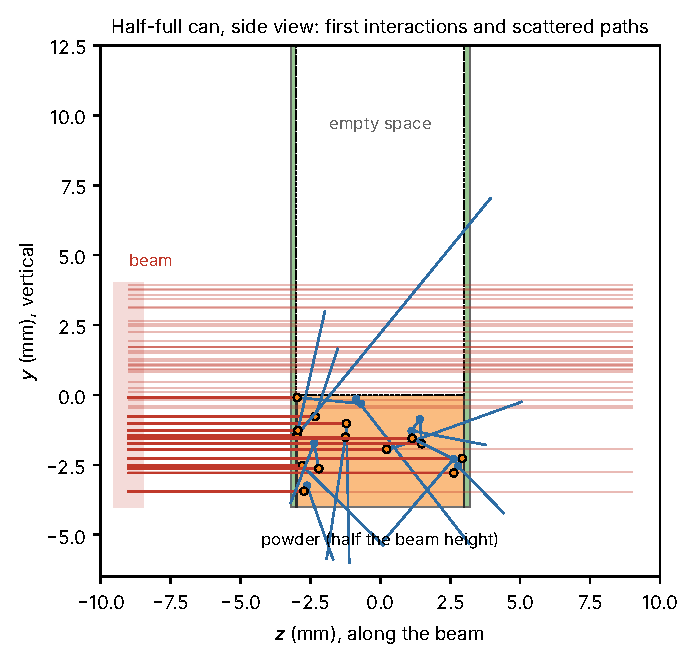
\includegraphics[width=0.78\textwidth]{fig_partial_trajectories}
  \caption{Half-full can in side view (projection on the vertical plane of the beam). Red: incident particles; the faint
  lines are particles that do not interact, most of them above the powder. Dots: first interactions. Blue: the following
  scattering events and the final exit; some particles go up into the empty space, cross it and hit the wall or leave
  through the top.}
  \label{fig:partialtraj}
\end{figure}

\section{Results}
\label{sec:partial-results}

Figure~\ref{fig:partialfull} shows what happens in the example can (powder $\mu=0.25$~mm$^{-1}$, scatter fraction 0.8;
vanadium wall 0.2~mm, $\mu=0.073$~mm$^{-1}$, scatter fraction 0.5; beam $8\times8$~mm, bottom of the can at the bottom of the beam)
as a function of the fullness, with $4\times10^5$ incident particles per point.

\begin{figure}[H]
  \centering
  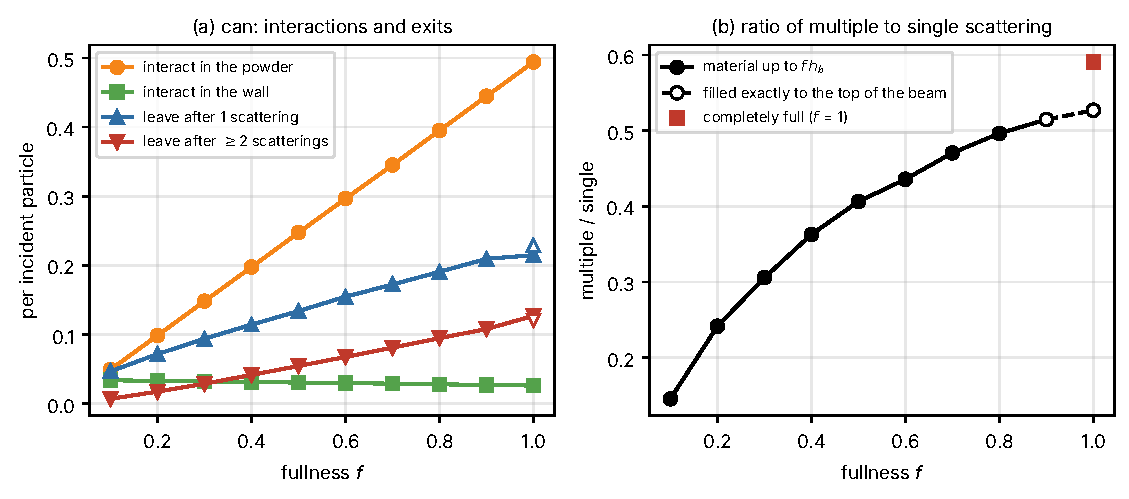
\includegraphics[width=\textwidth]{fig_partial_fullness}
  \caption{Example can versus fullness. (a)~Fraction of the incident particles that interact in the powder and in the wall,
  and that leave the sample after one or after two or more scatterings. Open symbols: can filled exactly up to the top
  of the beam ($h=h_b$). (b)~Ratio of multiple to single scattering.}
  \label{fig:partialfull}
\end{figure}

\begin{itemize}
  \item The scattering in the powder is proportional to the fullness, but the \textbf{multiple scattering grows faster}: the
        ratio of multiple to single scattering goes from 0.15 at $f=0.1$ to 0.52 at $f=0.9$. A thin layer of powder has few
        neighbours to scatter the particles again.
  \item Between ``filled exactly up to the top of the beam'' and ``completely full'' the illuminated material is the same, yet
        the ratio goes from 0.53 to 0.59, and the single scattering leaving the sample decreases (0.229 to 0.215 per incident particle).
        The material \emph{above} the beam scatters again, or absorbs, the particles that go upwards. This is why
        \code{fullness=1} (completely full) and \code{fill_height=beam_height} are different samples.
  \item The wall scatters slightly more when the can empties, because the downstream wall is no longer in the shadow of the
        powder.
\end{itemize}

\paragraph{Position of the material.} Figure~\ref{fig:bandpos} moves a band of powder 4~mm high through the 8~mm beam,
in a can from $-15$ to $+15$~mm. The interactions in the powder, and the single scattering that leaves the sample, follow the
fullness of eq.~(\ref{eq:fullness-general}), as expected. The ratio of multiple to single scattering does not: it is constant
(0.41) while the whole band is inside the beam, and drops to 0.28 when only an edge of the band is illuminated. Particles that
interact near the edge of the material have fewer neighbours to scatter them again. Two samples with the same fullness can
therefore have different multiple scattering.

\begin{figure}[H]
  \centering
  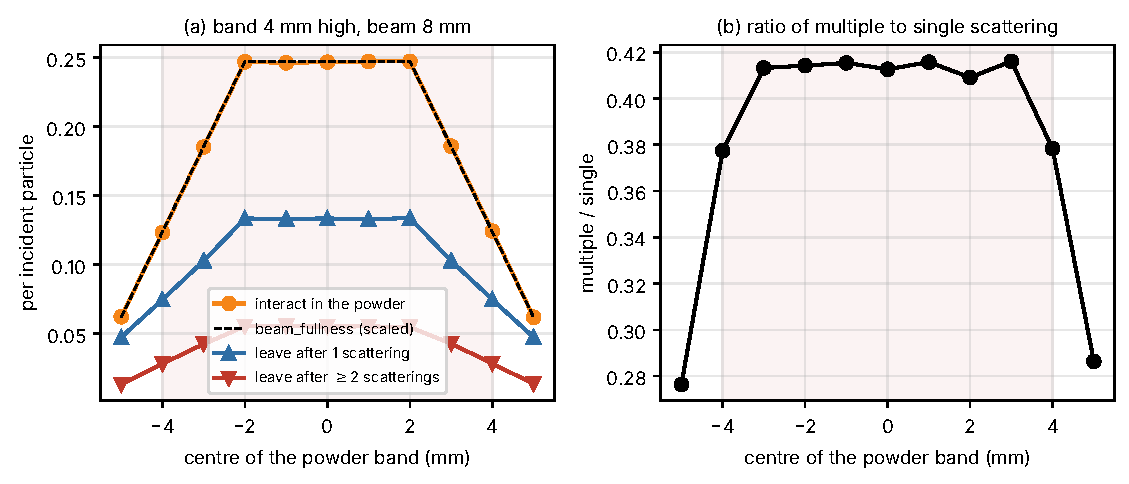
\includegraphics[width=\textwidth]{fig_band_position}
  \caption{A band of powder 4~mm high (example powder, $\mu=0.25$~mm$^{-1}$) moved through an $8\times8$~mm beam (shaded), inside a
  V can from $-15$ to $+15$~mm, $3\times10^5$ particles per point. (a)~Interactions in the powder, the fullness (scaled), and the
  particles that leave after one or more scatterings. (b)~Ratio of multiple to single scattering.}
  \label{fig:bandpos}
\end{figure}

The transmission of the scattered particles (Chapter~\ref{ch:transmission}) changes much less
(Figures~\ref{fig:partialtcyl} and~\ref{fig:partialtslab}). The detector of a two-axis instrument is in the horizontal plane,
so a particle scattered towards it stays at the same height: if it was scattered in the powder, it crosses powder on the way
out whatever the fullness. The transmission increases at low fullness mainly because a larger share of the interactions takes
place in the weakly absorbing wall, above the powder. The partial filling therefore matters mostly through \emph{how much} and
\emph{where} the sample scatters, and through the multiple scattering, rather than through the attenuation of the singly
scattered particles.

\begin{figure}[H]
  \centering
  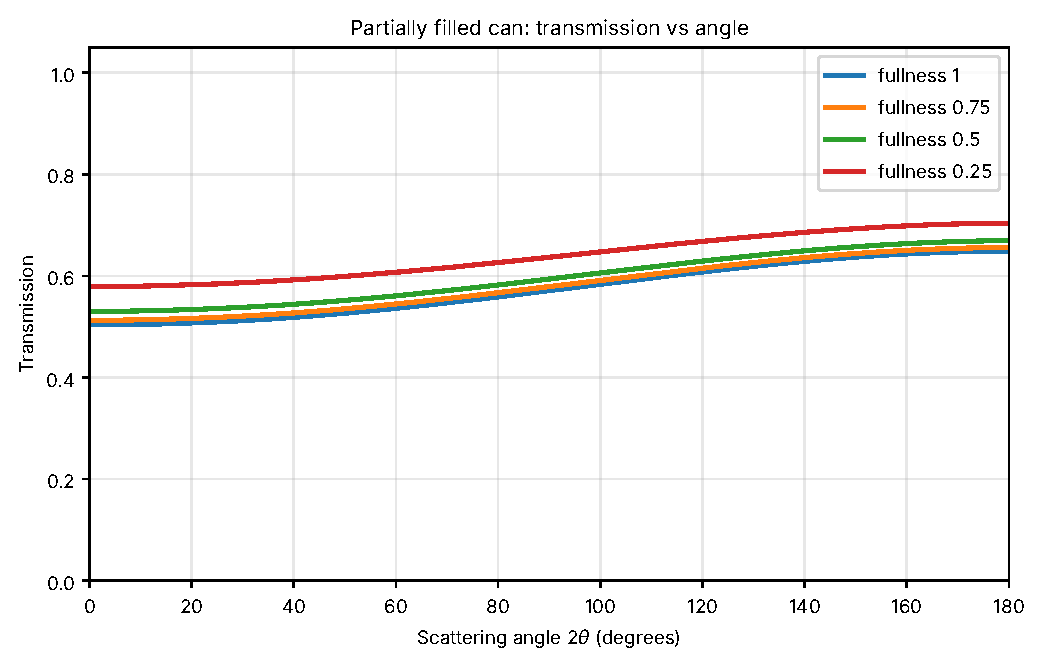
\includegraphics[width=0.78\textwidth]{fig_partial_transmission_cylinder}
  \caption{Example can: transmission versus $\twotheta$ for four values of the fullness.}
  \label{fig:partialtcyl}
\end{figure}

\begin{figure}[H]
  \centering
  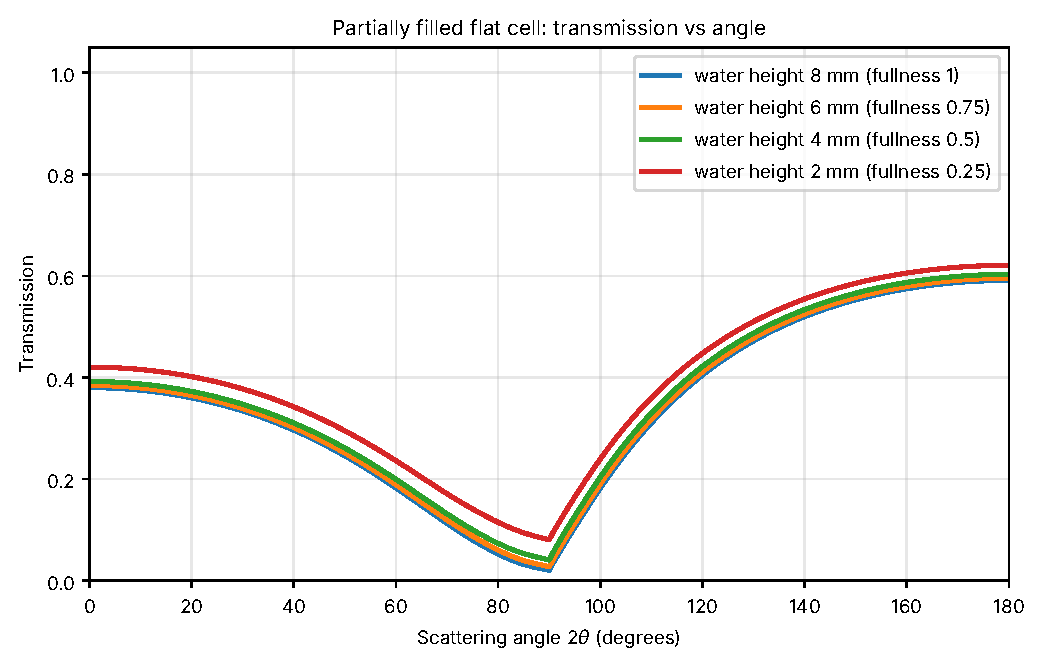
\includegraphics[width=0.78\textwidth]{fig_partial_transmission_slab}
  \caption{Flat cell perpendicular to the beam (aluminium windows of 1~mm, 3~mm of water with $\mu=0.56$~mm$^{-1}$), bottom
  at the bottom of the beam, for four heights of water. The minimum at $90^\circ$ is the direction parallel to the cell.}
  \label{fig:partialtslab}
\end{figure}

\section{With the main script}

\code{run_simulation.py} (Chapter~\ref{ch:main}) has the options \code{--bottom} and \code{--height} (version 2.2), and
\code{--fullness} (version 2.0). They set the band of the layers whose names are listed in \code{CONTENT_LAYERS}, at the top
of the file; the other layers (the walls) stay full. The bottom of the sample is set by \code{SAMPLE_Y_BOTTOM} (default
\code{None}: centred on the beam).
\begin{lstlisting}[style=shell]
python run_simulation.py --geometry cylinder --bottom -6 --height 5
python run_simulation.py --geometry cylinder --fullness 0.5
\end{lstlisting}
\begin{lstlisting}
results = run_simulation("cylinder", bottom=-6, height=5, show=False)
results = run_simulation("cylinder", fullness=0.5, show=False)
\end{lstlisting}
The names of the plot files then end with the band or the fullness, for example\\
\file{transmission\_cylinder\_b-6\_h5.png} or \file{transmission\_cylinder\_full0.5.png}.

\section{Assumptions}

\begin{itemize}
  \item The upper surface of the material is a \textbf{flat horizontal plane}: no meniscus, no slope of a powder. A slab rotated around
        the vertical axis keeps a horizontal surface, as a real cell would.
  \item The space above the material is \textbf{empty} ($\mu=0$). A gas can be added only as a separate full layer.
  \item The surfaces that limit the material are \textbf{horizontal planes} ($y=b_i$ and $y=t_i$). The same holds below the material:
        the band of a powder resting on a support starts at a flat horizontal surface.
  \item The bottom and the lid of a container, and a support, are not layers: the layers of a slab are perpendicular to its normal,
        and those of a cylinder are concentric. A support can be described only by its effect, the empty space below the material.
        A particle reaching the bottom or the top of the sample leaves it.
\end{itemize}
